\mode*
\part{Interprocess Communication}
\lecture{IPC}{ipc}

\begin{itemize}
\item \url{https://stackoverflow.com/questions/2281204/which-linux-ipc-technique-to-use}
\item \url{https://stackoverflow.com/questions/404604/comparing-unix-linux-ipc}
\item \url{https://www.thegeekstuff.com/2010/08/ipcs-command-examples/}
\end{itemize}

\begin{frame}{Interprocess Communication}
  \begin{iblock}{Example:}
    \begin{itemize}
    \item[\$] \cmd{unicode skull | head -1 | cut -f1 -d' ' | sm -}
    \end{itemize}
  \end{iblock}
  \begin{block}{IPC issues:}
    \begin{enumerate}
    \item How one process can pass information to another
    \item Be sure processes do not get into each other's way
      \begin{itemize}
      \item[e.g.] in an airline reservation system, two processes compete for the last
        seat
      \end{itemize}
    \item Proper sequencing when dependencies are present
      \begin{itemize}
      \item[e.g.] if A produces data and B prints them, B has to wait until A has produced
        some data
      \end{itemize}
    \end{enumerate}
  \end{block}
  \begin{block}{Two models of IPC:}
    \begin{itemize}
    \item Shared memory
    \item Message passing (e.g. sockets)
    \end{itemize}
  \end{block}
\end{frame}

\begin{frame}{Producer-Consumer Problem}
  \centering
  \mode<beamer>{ 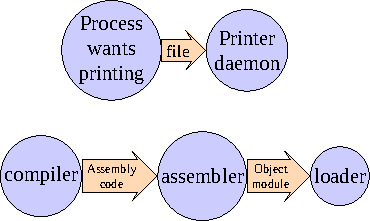
\includegraphics[width=.9\textwidth]{ipc} }%
  \mode<article>{ 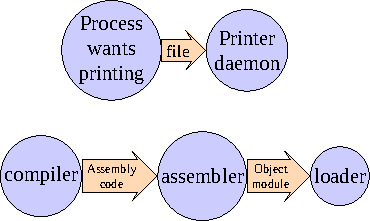
\includegraphics[width=.4\textwidth]{ipc} }
\end{frame}

\begin{frame}{Producer-Consumer Problem}
  \begin{itemize}
  \item Consumers don't try to remove objects from Buffer when it is empty.
  \item Producers don't try to add objects to the Buffer when it is full.
  \end{itemize}
  \begin{center}
    \mode<beamer>{ \includegraphics[width=\textwidth]{producer-consumer} }%
    \mode<article>{ \includegraphics[width=.5\textwidth]{producer-consumer-bw} }
  \end{center}
  \begin{center}
    How to define \alert{full/empty}?
  \end{center}
\end{frame}

\begin{frame}{Bounded-Buffer Problem (Circular Array)}
  \begin{minipage}{.65\linewidth}
  \begin{description}
  \item[Front(out):] the first full position
  \item[Rear(in):] the next free position
  \end{description}
  \end{minipage}\quad
  \begin{minipage}{.3\linewidth}
    \mode<beamer>{ 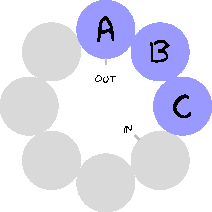
\includegraphics[width=\textwidth]{circular} }%
    \mode<article>{ 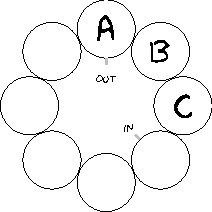
\includegraphics[width=.7\textwidth]{circular-bw} }
  \end{minipage}
  Full or empty when ``$front == rear$''?
\end{frame}

\begin{frame}
  \begin{block}{Common solution:}
    \begin{description}
    \item[Full:] when ``$\mathtt{(in+1)\%BUFFER\_SIZE == out}$''
      \begin{itemize}
      \item[] Actually, this is ``$\mathtt{full - 1}$''
      \end{itemize}
    \item[Empty:] when ``$\mathtt{in == out}$''
    \end{description}
    Can only use ``$\mathtt{BUFFER\_SIZE-1}$'' elements
  \end{block}  
  \begin{iblock}{Shared data:}
    \begin{center}
      \mode<beamer>{ \includegraphics[width=.8\textwidth]{shared-data} }%
      \mode<article>{ \includegraphics[width=.4\textwidth]{shared-data-bw} }
    \end{center}
  \end{iblock}
\end{frame}

\begin{frame}{Bounded-Buffer Problem}
  \begin{minipage}{.45\linewidth}
    \begin{iblock}{Producer:}
        \mode<beamer>{ \includegraphics[width=\textwidth]{bounded-buffer-1} }%
        \mode<article>{ 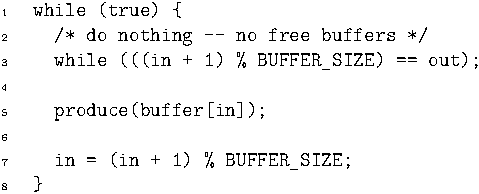
\includegraphics[width=.8\textwidth]{bounded-buffer-1-bw} }
    \end{iblock}
    \begin{iblock}{Consumer:}
      \mode<beamer>{ 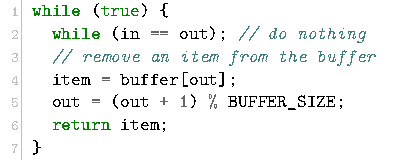
\includegraphics[width=\textwidth]{bounded-buffer-2} }%
      \mode<article>{ \includegraphics[width=.8\textwidth]{bounded-buffer-2-bw} }
    \end{iblock}
  \end{minipage}\hfill
  \begin{minipage}{.35\linewidth}
    \mode<beamer>{ 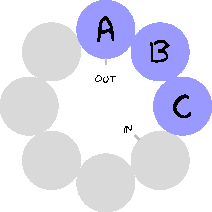
\includegraphics[width=\textwidth]{circular} }%
    \mode<article>{ 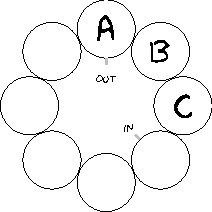
\includegraphics[width=\textwidth]{circular-bw} }
  \end{minipage}
\end{frame}

\section{Pipes and FIFOs}
\label{sec:pipes-fifos}

\begin{itemize}
\item \citetitle[chap.~44]{kerrisk:2010:lpi:1869911}
\end{itemize}

\begin{frame}{Pipe}
  \begin{itemize}
  \item[\$] \cmd{ls | wc -l}
  \end{itemize}
  \centering%
  \mode<beamer>{ 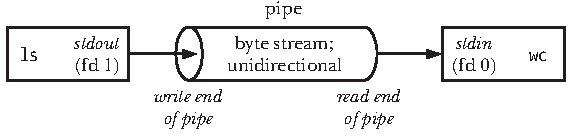
\includegraphics[width=.65\textwidth]{pipe-ls-wc} }%
  \mode<article>{ 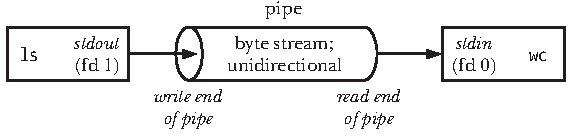
\includegraphics[width=.6\textwidth]{pipe-ls-wc} }

  \begin{itemize}
  \item A pipe is a byte stream
  \item Unidirectional
  \item \texttt{read()} would be blocked if nothing written at the other end
  \end{itemize}
  \ttfamily
  \begin{iblock}{\texttt{tee}}
    \begin{minipage}{.35\linewidth}
      \begin{itemize}
      \item[\$] ls | tee ls.out
      \end{itemize}
    \end{minipage}\quad
    \begin{minipage}{.45\linewidth}
      \mode<beamer>{ 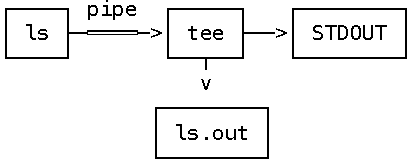
\includegraphics[width=\textwidth]{tee} }%
      \mode<article>{ 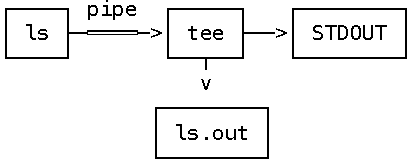
\includegraphics[width=.6\textwidth]{tee} }
    \end{minipage}
  \end{iblock}
\end{frame}

\begin{itemize}
\item When we say that a pipe is a byte stream, we mean that there is no concept of
  messages or message boundaries when using a pipe. The process reading from a pipe can
  read blocks of data of any size, regardless of the size of blocks written by the writing
  process. Furthermore, the data passes through the pipe sequentially --- bytes are read from
  a pipe in exactly the order they were written. It is not possible to randomly access the
  data in a pipe using \texttt{lseek()}. \citetitle[chap.~44]{kerrisk:2010:lpi:1869911}
\end{itemize}


\begin{frame}
\begin{center}
  \mode<beamer>{ 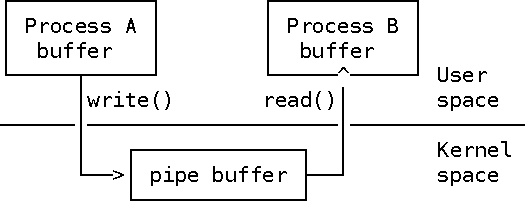
\includegraphics[width=.6\textwidth]{pipe} }%
  \mode<article>{ 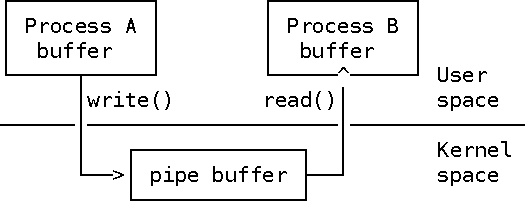
\includegraphics[width=.4\textwidth]{pipe} }
\end{center}
\begin{itemize}
\item No direct link between A and B (need system calls)
\item A pipe is simply a buffer maintained in kernel memory
  \begin{itemize}
  \item[\$] \cmd{cat /proc/sys/fs/pipe-max-size}
  \end{itemize}
\end{itemize}
\end{frame}

\begin{frame}{\texttt{pipe()}}
  \begin{minipage}{.3\linewidth}
    \mode<beamer>{ \includegraphics[width=\textwidth]{pipe-prototype-c} }%
    \mode<article>{\cfile{../src/pseudo/pipe-prototype.c}}
  \end{minipage}\quad
  \begin{minipage}{.3\linewidth}
    \mode<beamer>{ \includegraphics[width=\textwidth]{pipe1} }%
    \mode<article>{ \includegraphics[width=.8\textwidth]{pipe1} }
  \end{minipage}

  \begin{description}
  \item[\texttt{pipe()} + \texttt{fork()}]
  \end{description}
  \centering%
  \mode<beamer>{ 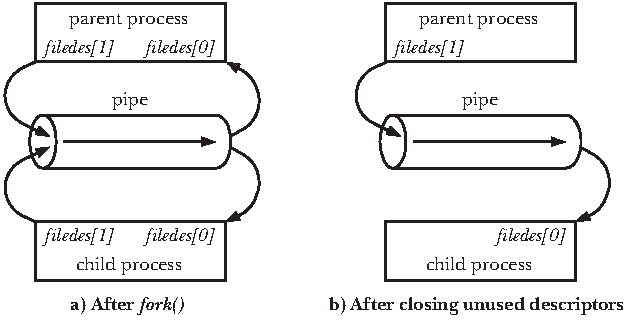
\includegraphics[width=.6\textwidth]{pipe2} }%
  \mode<article>{ 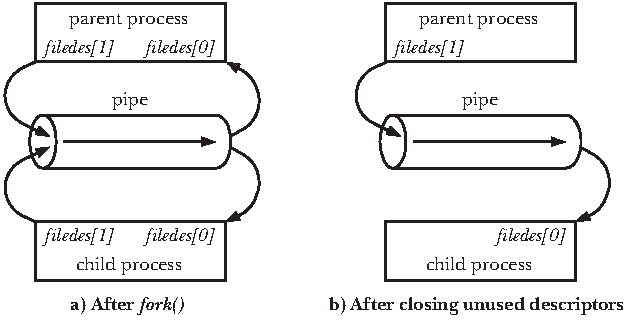
\includegraphics[width=.5\textwidth]{pipe2} }
\end{frame}

\begin{itemize}
\item Pipes must have a reader and a writer. If a process tries to write to a pipe that
  has no reader, it will be sent the SIGPIPE signal from the kernel. This is imperative
  when more than two processes are involved in a
  pipeline. (\url{http://www.tldp.org/LDP/lpg/node20.html})
\item While it is possible for the parent and child to both read from and write to the
  pipe, this is not usual. Therefore, immediately after the \texttt{fork()}, one process
  closes its descriptor for the write end of the pipe, and the other closes its descriptor
  for the read end. For example, if the parent is to send data to the child, then it would
  close its read descriptor for the pipe, \texttt{filedes[0]}, while the child would close
  its write descriptor for the pipe, \texttt{filedes[1]}.
  
  One reason that it is not usual to have both the parent and child reading from a single
  pipe is that if two processes try to simultaneously read from a pipe, we can't be sure
  which process will be the first to succeed—the two processes race for data.  Preventing
  such races would require the use of some synchronization mechanism.  However, if we
  require bidirectional communication, there is a simpler way: just create two pipes, one
  for sending data in each direction between the two processes.  (If employing this
  technique, then we need to be wary of deadlocks that may occur if both processes block
  while trying to read from empty pipes or while trying to write to pipes that are already
  full.) \citetitle[chap.~44, p.~893]{kerrisk:2010:lpi:1869911}
\item Pipes can be used for communication between any two (or more) related processes, as
  long as the pipe was created by a common ancestor before the series of \texttt{fork()}
  calls that led to the existence of the processes. For example, a pipe could be used for
  communication between a process and its grandchild. The first process creates the pipe,
  and then forks a child that in turn forks to yield the grandchild. A common scenario is
  that a pipe is used for communication between two siblings --- their parent creates the
  pipe, and then creates the two children. This is what the shell does when building a
  pipeline.
\item \textbf{Closing unused pipe file descriptors}. The process reading from the pipe
  closes its write descriptor for the pipe, so that, when the other process completes its
  output and closes its write descriptor, the reader sees end-of-file (once it has read
  any outstanding data in the pipe).  If the reading process doesn't close the write end
  of the pipe, then, after the other process closes its write descriptor, the reader won't
  see end-of-file, even after it has read all data from the pipe. Instead, a
  \texttt{read()} would block waiting for data, because the kernel knows that there is
  still at least one write descriptor open for the pipe. That this descriptor is held open
  by the reading process itself is irrelevant; in theory, that process could still write
  to the pipe, even if it is blocked trying to read.  For example, the \texttt{read()}
  might be interrupted by a signal handler that writes data to the pipe.

  The writing process closes its read descriptor for the pipe for a different reason.
  When a process tries to write to a pipe for which no process has an open read
  descriptor, the kernel sends the SIGPIPE signal to the writing process. By default, this
  signal kills a process. A process can instead arrange to catch or ignore this signal, in
  which case the \texttt{write()} on the pipe fails with the error EPIPE (broken
  pipe). Receiving the SIGPIPE signal or getting the EPIPE error is a useful indication
  about the status of the pipe, and this is why unused read descriptors for the pipe
  should be closed.

  If the writing process doesn't close the read end of the pipe, then, even after the
  other process closes the read end of the pipe, the writing process will still be able to
  write to the pipe. Eventually, the writing process will fill the pipe, and a further
  attempt to write will block indefinitely.

  One final reason for closing unused file descriptors is that it is only after all file
  descriptors in all processes that refer to a pipe are closed that the pipe is destroyed
  and its resources released for reuse by other processes. At this point, any unread data
  in the pipe is lost.
\end{itemize}

\begin{frame}
  \mode<beamer>{ 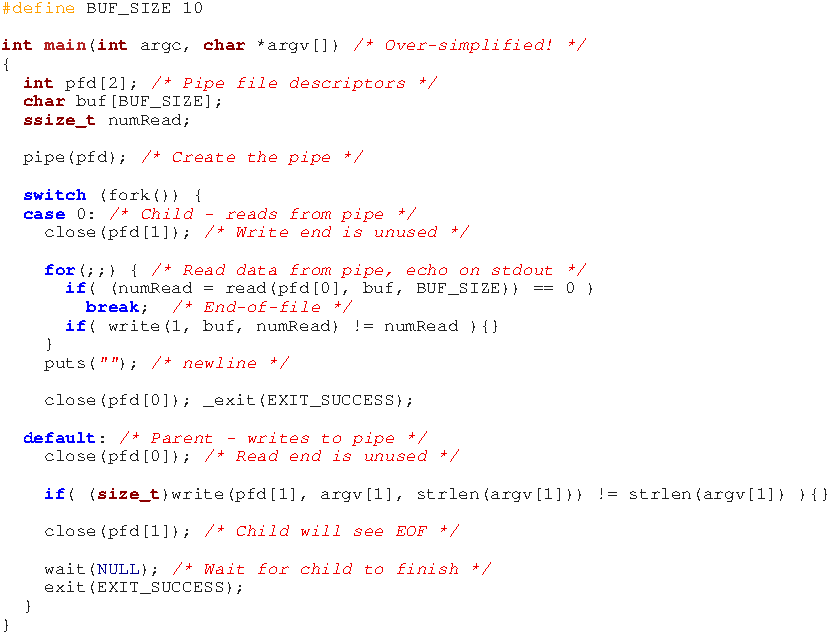
\includegraphics[height=\textheight]{simple_pipe-c} }%
  \mode<article>{\cfile{../src/simple_pipe.c}}
\end{frame}

\begin{itemize}
\item
  \url{https://stackoverflow.com/questions/5422831/what-is-the-difference-between-using-exit-exit-in-a-conventional-linux-fo}
\item \texttt{\_exit(2)}
\end{itemize}

\begin{frame}{\texttt{popen()}}
\begin{center}
  \mode<beamer>{ 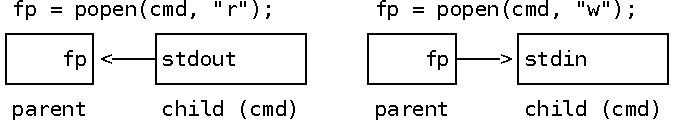
\includegraphics[width=.8\textwidth]{popen} }%
  \mode<article>{ 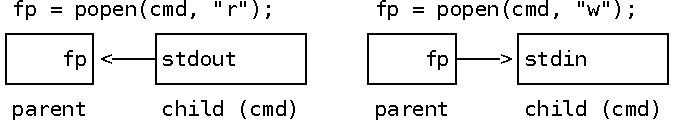
\includegraphics[width=.6\textwidth]{popen} }
\end{center}
\begin{description}
\item[\texttt{popen()}] does a \texttt{fork()} and \texttt{exec()} to execute the
  \texttt{cmd} and returns STD I/O file pointer.
  \begin{itemize}
  \item[r] \texttt{fp} is readable (stdout)
  \item[w] \texttt{fp} is writable (stdin)
  \end{itemize}
\end{description}
\end{frame}

\begin{itemize}
\item \citetitle[Sec.~15.3]{stevens2013advanced}
\item \citetitle[Sec.~13.2]{matthew2008beginning}
\end{itemize}

\begin{frame}{Example}
  \centering%
  \mode<beamer>{ 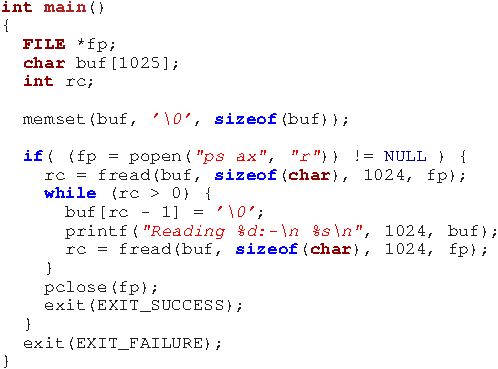
\includegraphics[width=.7\textwidth]{popen3} }%
  \mode<article>{\cfile{../src/popen3.c}}

  \begin{itemize}
  \item[\$] \cmd{ps ax | cat}
  \end{itemize}
\end{frame}

\begin{frame}{Example}
  \centering%
  \mode<beamer>{ 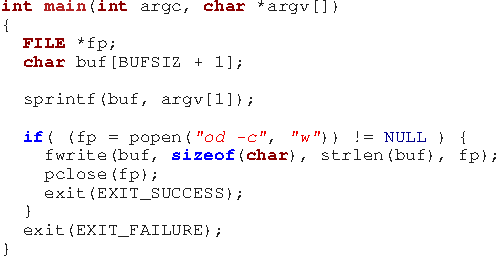
\includegraphics[width=.8\textwidth]{popen2} }%
  \mode<article>{\cfile{../src/popen2.c}}
  \begin{itemize}
  \item[\$] \cmd{echo -n hello | od -c}
  \end{itemize}
\end{frame}


\begin{frame}{Named Pipe (FIFO)}
  \begin{description}
  \item[PIPEs] pass data between related processes.
  \item[FIFOs] pass data between any processes.
  \end{description}
  \begin{iblock}{\CMD{mkfifo myfifo}}
    \begin{center}
      \begin{minipage}{.45\linewidth}\ttfamily
        \begin{itemize}
        \item[\$] echo hello > myfifo
        \item[\$] cat myfifo
        \end{itemize}
      \end{minipage}\quad
      \begin{minipage}{.5\linewidth}
        \mode<beamer>{ 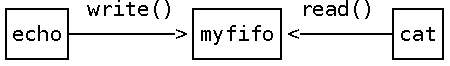
\includegraphics[width=\textwidth]{fifo} }%
        \mode<article>{ 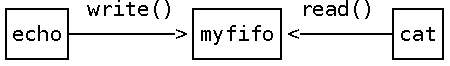
\includegraphics[width=.6\textwidth]{fifo} }
      \end{minipage}
    \end{center}
  \end{iblock}
  \ttfamily
  \begin{iblock}{\texttt{tee}}
    \begin{minipage}{.5\linewidth}
      \begin{itemize}
      \item[\$] echo hello | tee myfifo
      \item[\$] wc myfifo
      \end{itemize}
    \end{minipage}\quad
    \begin{minipage}{.45\linewidth}
      \mode<beamer>{ 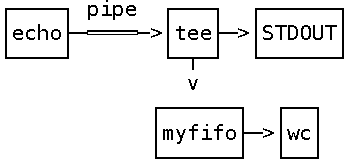
\includegraphics[width=\textwidth]{fifo-tee} }%
      \mode<article>{ 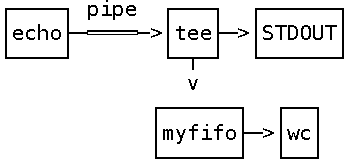
\includegraphics[width=.6\textwidth]{fifo-tee} }
    \end{minipage}
  \end{iblock}
\end{frame}

\begin{itemize}
\item \url{https://en.wikipedia.org/wiki/Named_pipe}
\end{itemize}

\begin{frame}{IPC With FIFO}
  \mode<beamer>{ 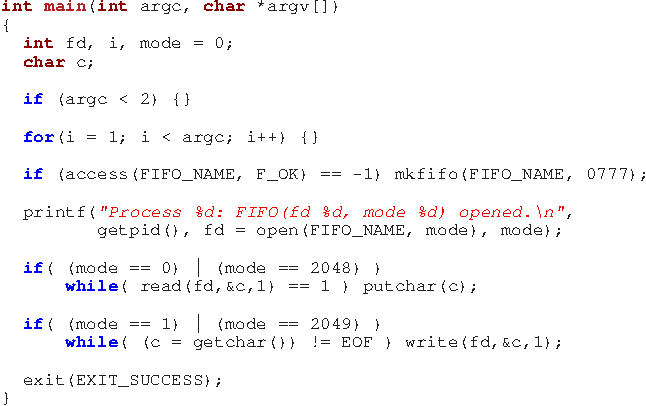
\includegraphics[height=.9\textheight]{fifo2-ipc} }%
  \mode<article>{\cfile{../src/fifo2.c}}
\end{frame}

\begin{frame}
  {\ttfamily
    \begin{itemize}
    \item[\$] watch 'lsof -n.1 /tmp/myfifo'
    \item[\$] ./a.out O\_RDONLY
    \item[\$] ./a.out O\_WRONLY
    \item[\$] ./a.out O\_RDONLY O\_NONBLOCK
    \item[\$] ./a.out O\_WRONLY O\_NONBLOCK
    \end{itemize}}
  \begin{block}{\texttt{O\_NONBLOCK}}
    \begin{itemize}
    \item A \texttt{read()/write()} will wait on an empty blocking FIFO
    \item A \texttt{read()} on an empty nonblocking FIFO will return 0 bytes
    \item \cmd{open(const char *path, O\_WRONLY | O\_NONBLOCK);}
      \begin{itemize}
      \item Returns an error (-1) if FIFO not open
      \item Okay if someone's reading the FIFO
      \end{itemize}
    \item If opened with \texttt{O\_RDWR}, the result is undefined
    \end{itemize}
  \end{block}
\end{frame}

\begin{itemize}
\item If opened with \texttt{O\_RDWR}, the result is undefined. If you do want to pass
  data in both directions, it's much better to use a pair of FIFOs or pipes, one for each
  direction.
\item There are four legal combinations of \texttt{O\_RDONLY}, \texttt{O\_WRONLY}, and the
  \texttt{O\_NONBLOCK} flag. 
\end{itemize}
\begin{longlisting}
  \cfile{../src/pseudo/o_nonblock.c}
\end{longlisting}

\section{Message Queues}
\label{sec:message-queues}

\begin{frame}{Message Queues}
  \centering%
  \begin{minipage}{.2\linewidth}
    \mode<beamer>{ \includegraphics[width=\textwidth]{mq} }%
    \mode<article>{ \includegraphics[width=.6\textwidth]{mq} }
  \end{minipage}\qquad
  \begin{minipage}{.3\linewidth}
    \mode<beamer>{ 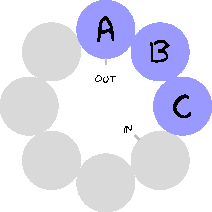
\includegraphics[width=\textwidth]{circular} }%
    \mode<article>{ 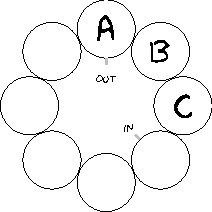
\includegraphics[width=.6\textwidth]{circular-bw} }
  \end{minipage}
\end{frame}

\begin{itemize}
\item \citetitle[Sec.~52.3]{kerrisk:2010:lpi:1869911}
\item \texttt{mq\_overview(7)}
\item \texttt{sem\_overview(7)}
\item \texttt{shm\_overview(7)}
\item \url{https://www.uninformativ.de/blog/postings/2016-05-16/0/POSTING-en.html}
\end{itemize}

\begin{frame}{Message Queues}{Send}
  \centering
  \mode<beamer>{ 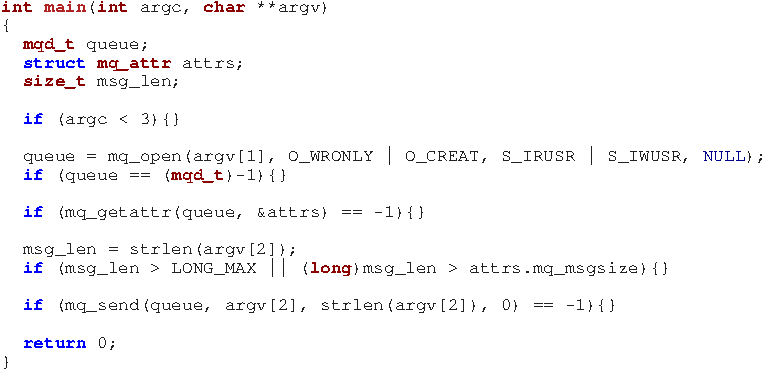
\includegraphics[width=\textwidth]{mq-send} }%
  \mode<article>{\cfile{../src/mq-send.c}}
\end{frame}

\begin{frame}{Message Queues}{Receive}
  \centering
  \mode<beamer>{ 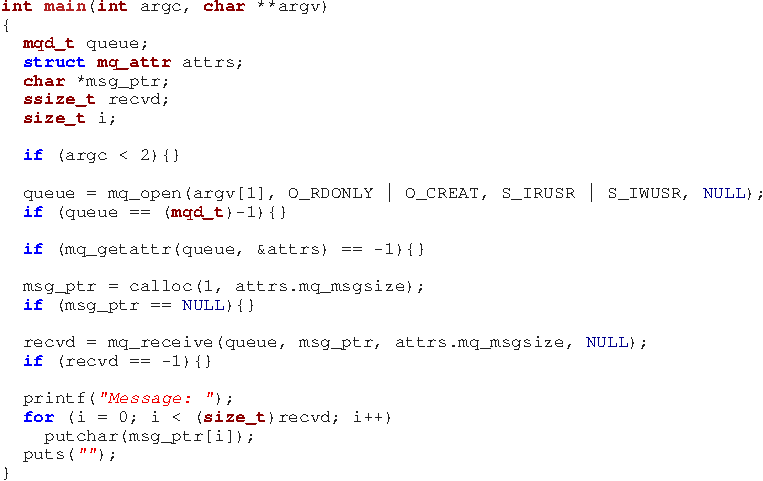
\includegraphics[height=.85\textheight]{mq-recv} }%
  \mode<article>{\cfile{../src/mq-recv.c}}
\end{frame}

\begin{frame}{Relationship Between Kernel Data Structures}
\begin{center}
  \mode<beamer>{ 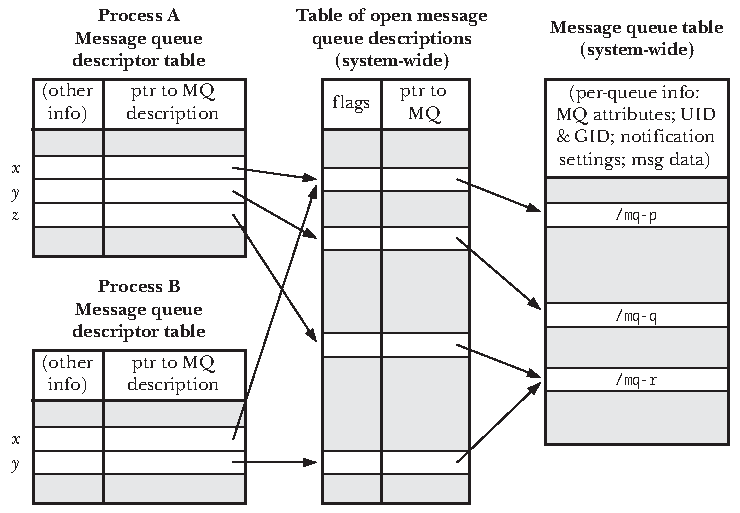
\includegraphics[width=.8\textwidth]{msgq} }%
  \mode<article>{ 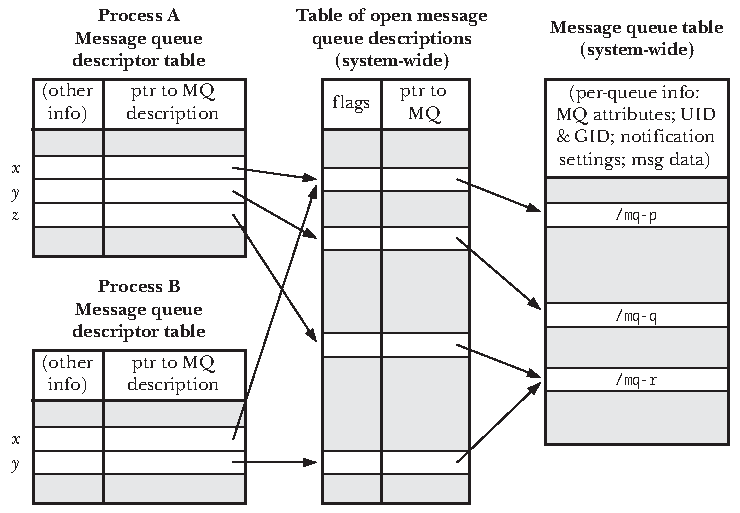
\includegraphics[width=.6\textwidth]{msgq} }
\end{center}
\end{frame}

\section{Semaphores}
\label{sec:semaphores}

\begin{frame}{Race Conditions}
  \centering
  \mode<beamer>{ 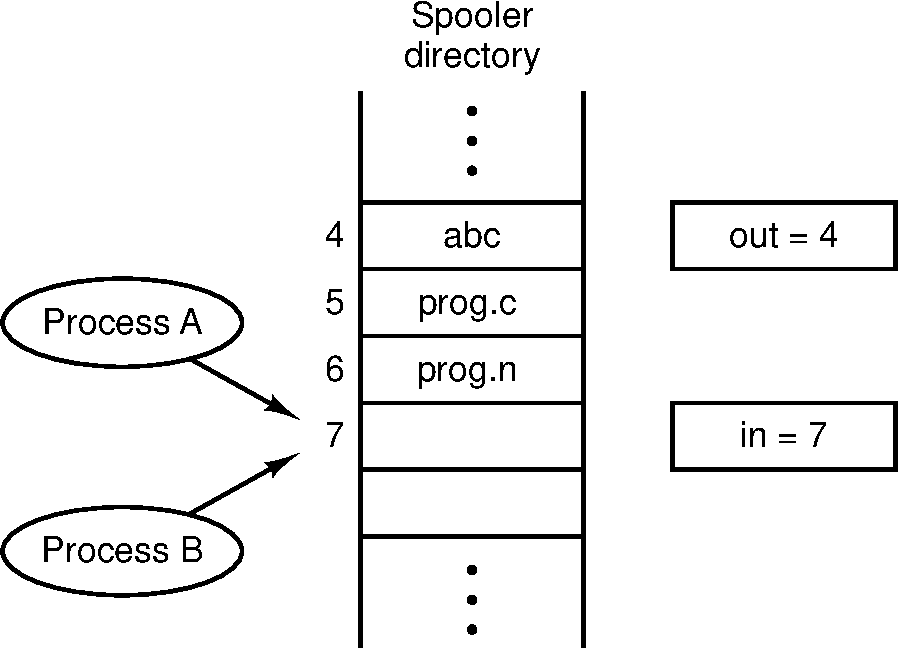
\includegraphics[width=.7\textwidth]{mos-figs-2-18} }%
  \mode<article>{ 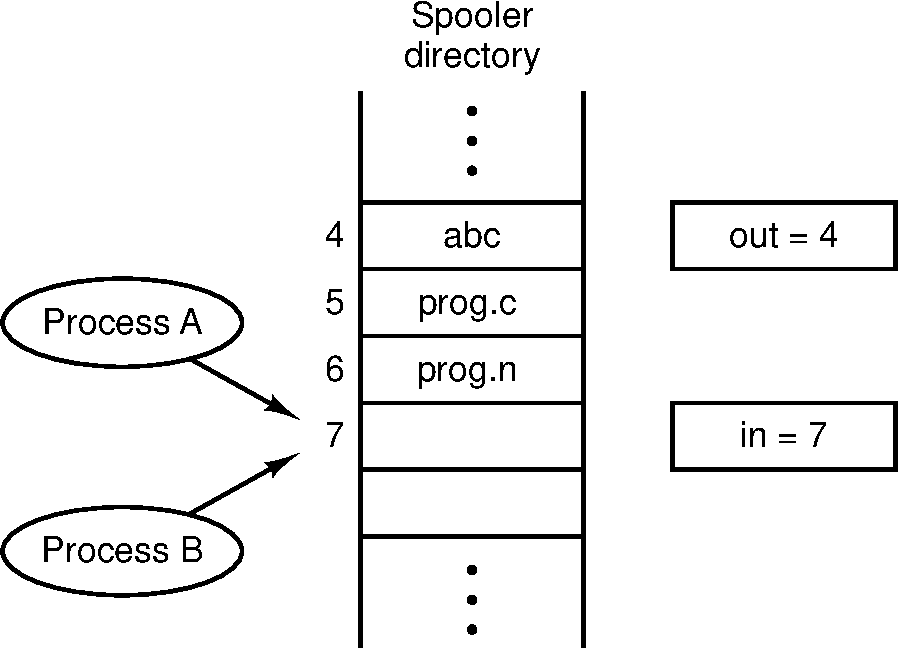
\includegraphics[width=.45\textwidth]{mos-figs-2-18} }
\end{frame}

\begin{frame}{Mutual Exclusion}
  \begin{description}
  \item[Critical Region] is a piece of code accessing a common resource.
  \end{description}
  \begin{center}
    \mode<beamer>{ 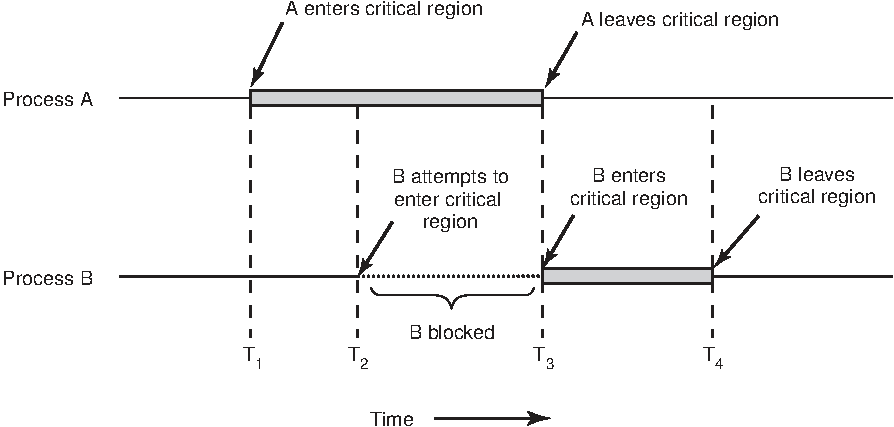
\includegraphics[width=\textwidth]{mos-figs-2-19} }%
    \mode<article>{ 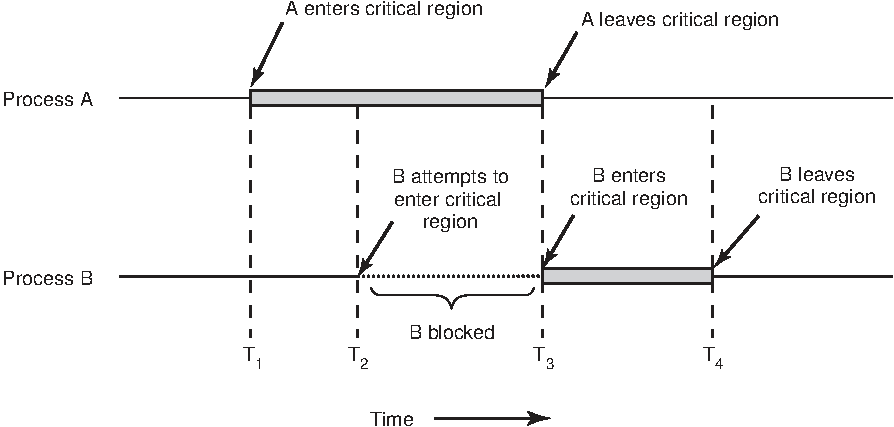
\includegraphics[width=.7\textwidth]{mos-figs-2-19} }
  \end{center}
\end{frame}

\begin{frame}
  \begin{block}{A solution to the critical region problem must satisfy three conditions}
    \begin{description}
    \item[Mutual Exclusion:] No two processes may be simultaneously inside their critical
      regions.
    \item[Progress:] No process running outside its critical region may block other
      processes.
    \item[Bounded Waiting:] No process should have to wait forever to enter its critical
      region.
    \end{description}
  \end{block}
\end{frame}

\begin{frame}{Mutual Exclusion With Busy Waiting}{Strict Alternation}
  \begin{center}
    \mode<beamer>{ 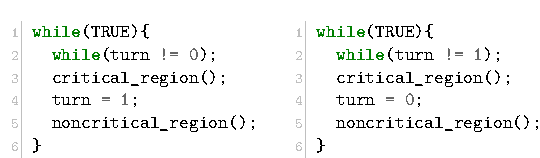
\includegraphics[width=\textwidth]{strict-alternation} }%
    \mode<article>{ \includegraphics[width=.5\textwidth]{strict-alternation-bw} }
  \end{center}
  \begin{itemize}
  \item[\Bad] One process can be blocked by another not in its critical region
  \end{itemize}
\end{frame}

\begin{frame}{Mutual Exclusion With Busy Waiting}{Peterson's Solution}
  \centering
  \mode<beamer>{ 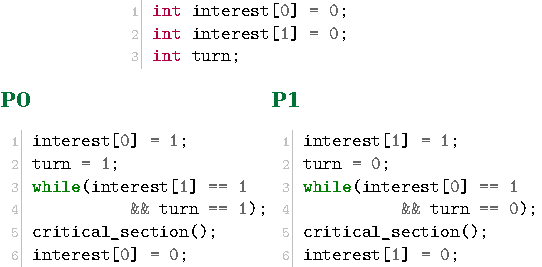
\includegraphics[width=.85\textwidth]{peterson} }%
  \mode<article>{ \includegraphics[width=.6\textwidth]{peterson-bw} }
  \begin{refsection}
    \nocite{wiki:peterson}
    \printbibliography[heading=none]
  \end{refsection}
\end{frame}

\begin{frame}{Mutual Exclusion With Busy Waiting}{Lock file}
  \mode<beamer>{ \includegraphics[width=\textwidth]{lock2-c} }%
  \mode<article>{\cfile{../src/lock2.c}}
  \begin{itemize}
  \item[\Bad] Lock file could be left in system after \Cc
  \end{itemize}
\end{frame}

\begin{frame}
  \mode<beamer>{ \includegraphics[width=.9\textwidth]{lock2-sigint-c} }%
  \mode<article>{\cfile{../src/lock2-sigint.c}}
  \begin{itemize}
  \item[\Bad] \texttt{sigint()} is too crude to be reliable. Need a more sophisticated design.
  \end{itemize}
\end{frame}

% \begin{itemize}
% \item The \texttt{sigint()} function is too crude to be reliable. 
% \end{itemize}

\begin{frame}{What is a Semaphore?\,\includegraphics[width=1em]{semaphore-papa}}
  \begin{minipage}{.5\linewidth}
    \begin{itemize}
    \item A locking mechanism
    \item An integer or ADT
    \end{itemize}
    \vspace*{2ex}
    \ttfamily\small
    \begin{tabular}{ll}\hline
      \multicolumn2{c}{\emph{Atomic} Operations}\\\hline
      P()         &V()\\
      Wait()      &Signal()\\
      Down()      &Up()\\
      Decrement() &Increment()\\
      ...         &...\\\hline
    \end{tabular}
  \end{minipage}\hfill
  \begin{minipage}{.45\linewidth}
    \mode<beamer>{ \includegraphics[width=\textwidth]{down-up} }%
    \mode<article>{ \includegraphics[width=\textwidth]{down-up-bw} }
  \end{minipage}
  \begin{iblock}{More meaningful names:}
    \begin{itemize}
    \item \texttt{increment\_and\_wake\_a\_waiting\_process\_if\_any()}
    \item \texttt{decrement\_and\_block\_if\_the\_result\_is\_negative()}
    \end{itemize}
  \end{iblock}
\end{frame}

\begin{frame}{Using Semaphore For Signaling}
  \begin{itemize}
  \item One thread sends a signal to another to indicate that something has
    happened
  \item It solves the serialization problem
    \begin{itemize}
    \item[] Signaling makes it possible to guarantee that a section of code in one thread
      will run before that in another
    \end{itemize}
  \end{itemize}
  \begin{center}
    \mode<beamer>{ \includegraphics[width=.7\textwidth]{sem-signaling} }%
    \mode<article>{ \includegraphics[width=.4\textwidth]{sem-signaling} }
  \end{center}
  \begin{center}
    What's the initial value of \texttt{sem}?
  \end{center}
\end{frame}

\begin{frame}{Example}% Signaling with semaphore
  \centering
  \mode<beamer>{ \includegraphics[height=.9\textheight]{thread3} }%
  \mode<article>{\cfile{../src/thread3.c}}
\end{frame}

\begin{itemize}
\item \citetitle[Sec.~12.5]{matthew2008beginning}
\item \url{https://stackoverflow.com/questions/368322/differences-between-system-v-and-posix-semaphores}
\end{itemize}

\begin{frame}{\texttt{i++} {\small can go wrong!}}
  \centering
  \mode<beamer>{ \includegraphics[height=.9\textheight]{atomic-non} }%
  \mode<article>{\cfile{../src/atomic-non.c}}
\end{frame}

\begin{frame}{Atomic}
  \begin{iblock}{\texttt{i++} is not atomic in assembly language}
    \begin{center}
      \mode<beamer>{ \includegraphics[width=.8\textwidth]{ipp} }%
      \mode<article>{ \includegraphics[width=.5\textwidth]{ipp-bw} }
    \end{center}
  \end{iblock}
  Interrupts might occur in between. So, \texttt{i++} needs to be protected with a \texttt{mutex}.
\end{frame}

\begin{frame}
  \begin{description}
  \item[Mutex] A semaphore that is initialized to 1. In case of:
    \begin{itemize}
    \item[1:] A thread may proceed and access the shared variable
    \item[0:] It has to wait for another thread to release the mutex
    \end{itemize}
  \end{description}
  \begin{center}
    \mode<beamer>{ \includegraphics[width=.8\textwidth]{mutex-ipp} }%
    \mode<article>{ \includegraphics[width=.5\textwidth]{mutex-ipp} }
  \end{center}
\end{frame}

\begin{frame}
  \centering%
  \mode<beamer>{ \includegraphics[height=\textheight]{atomic-mutex} }%
  \mode<article>{\cfile{../src/atomic-mutex.c}}
\end{frame}

\begin{frame}
\begin{center}
  \mode<beamer>{ \includegraphics[width=.7\textwidth]{mutex} }%
  \mode<article>{\cfile{../src/mutex.c}}
\end{center}
\end{frame}

\begin{frame}{Barrier}
  % the little book of semaphores
  \centering
  \mode<beamer>{ \includegraphics[width=.6\textwidth]{barrier} }%
  \mode<article>{ \includegraphics[width=.6\textwidth]{barrier} }

  {\small
  \begin{enumerate}
  \item Processes approaching a barrier
  \item All processes but one blocked at the barrier
  \item When the last process arrives at the barrier, all of them are let through
  \end{enumerate}}

  \begin{iblock}{Synchronization requirement:}
    \begin{center}\ttfamily
      \begin{tabular}{l}
        specific\_task()\\
        critical\_point()
      \end{tabular}
    \end{center}
    No thread executes \texttt{critical\_point()} until after all threads have executed
    \texttt{specific\_task()}.
  \end{iblock}
\end{frame}

\begin{frame}{Barrier Solution}
  \begin{minipage}{.38\linewidth}
    \mode<beamer>{ \includegraphics[width=\textwidth]{barrier-1} }%
    \mode<article>{ \includegraphics[width=.4\textwidth]{barrier-1} }
  \end{minipage}\hfill
  \begin{minipage}{.6\linewidth}
    \footnotesize%
    \begin{description}
    \item[count:] keeps track of how many threads have arrived
    \item[mutex:] provides exclusive access to \texttt{count}
    \item[barrier:] is locked ($\le 0$) until all threads arrive
    \end{description}
  \end{minipage}
  \vspace*{2ex}
  \begin{description}
  \item[When \texttt{barrier.value < 0},] \,\\
    \ttfamily barrier.value == Number of queueing processes
  \end{description}

  \begin{center}
    \mode<beamer>{ \includegraphics[width=.7\textwidth]{barrier-2} }%
    \mode<article>{ \includegraphics[width=.5\textwidth]{barrier-2-bw} }
    \pause%
    \alert{Only one thread can pass the barrier!}
  \end{center}
  
  \mode<beamer>{
    \begin{tikzpicture}[remember picture, overlay]
      \node [scale=10,text opacity=0.3,color=red,yshift=-.4em,xshift=-.4em] at (current
      page.center) {\Symbol{✔}};

      \node [scale=2.2,text opacity=0.3,color=red,yshift=-1.5em,xshift=3em,rotate=20] at
      (current page.center) {Deadlock!};
    \end{tikzpicture}}
\end{frame}

\begin{frame}{Barrier Solution}
  \centering
  \mode<beamer>{ \includegraphics[width=.8\textwidth]{barrier-3} }%
  \mode<article>{ \includegraphics[width=.5\textwidth]{barrier-3-bw} }

  \mode<beamer>{ \pause
    {\centering
      {\danger} \alert{Blocking on a semaphore while holding a
        mutex!} {\danger}}

    \begin{tikzpicture}[remember picture, overlay]
      \node [rotate=40,scale=3.5,text opacity=0.3,color=red,xshift=2.2em,yshift=-1em] at
      (current page.center) {Deadlock!};
    \end{tikzpicture}}%
  \mode<article>{
    \centering \danger{} Blocking on a semaphore while holding a mutex!\danger{}}
\end{frame}

\begin{frame}%{Barrier Solution}
  \begin{center}\ttfamily
    \begin{tabular}{l}
      barrier.wait();\\
      barrier.signal();
    \end{tabular}
  \end{center}
  \begin{block}{Turnstile}
    This pattern, a \texttt{wait} and a \texttt{signal} in rapid succession, occurs often
    enough that it has a name called a \emph{turnstile}, because
    \begin{itemize}
    \item it allows one thread to pass at a time, and
    \item it can be locked to bar all threads
    \end{itemize}
  \end{block}
\end{frame}

\section{Classical IPC Problems}
\label{sec:class-ipc-probl}

\subsection{The Dining Philosophers Problem}
\label{sec:dining-phil-probl}

\begin{frame}{The Dining Philosophers Problem}
  \begin{center}
    \begin{minipage}{.4\linewidth}
      \mode<beamer>{ \includegraphics[width=\textwidth]{dining} }%
      \mode<article>{ \includegraphics[width=.5\textwidth]{dining-bw} }
    \end{minipage} \qquad
    \begin{minipage}{.5\linewidth}
      \mode<beamer>{ \includegraphics[width=.7\textwidth]{dphil-0} }%
      \mode<article>{ \includegraphics[width=.4\textwidth]{dphil-0} }
    \end{minipage}
  \end{center}
  How to implement \texttt{get\_forks()} and \texttt{put\_forks()} to ensure
  \begin{enumerate}
  \item No deadlock
  \item No starvation
  \item Allow more than one philosopher to eat at the same time
  \end{enumerate}
\end{frame}

\begin{frame}{The Dining Philosophers Problem}{Deadlock}
  \begin{center}
    \mode<beamer>{ \includegraphics[width=\textwidth]{mos-figs-2-32} }%
    \mode<article>{ \includegraphics[width=.7\textwidth]{mos-figs-2-32} }
  \end{center}
  \begin{itemize}
  \item Put down the left fork and wait for a while if the right one is not available?
    Similar to CSMA/CD --- Starvation
  \end{itemize}
\end{frame}

\begin{frame}{The Dining Philosophers Problem}{With One Mutex}
  \begin{minipage}{.5\linewidth}
    \centering
      \mode<beamer>{ \includegraphics[width=\textwidth]{dining-mutex} }%
      \mode<article>{ \includegraphics[width=.7\textwidth]{dining-mutex-bw} }
  \end{minipage} \hfill
  \begin{minipage}{.45\linewidth}
    \centering%
    \mode<beamer>{ \includegraphics[width=.6\textwidth]{dphil-0} }%
    \mode<article>{ \includegraphics[width=.5\textwidth]{dphil-0} } \pause
    \begin{itemize}
    \item[\Bad] Only one philosopher can eat at a time.
    \item[?] How about 2 mutexes, 5 mutexes?
    \end{itemize}
  \end{minipage}
\end{frame}

\begin{frame}{The Dining Philosophers Problem}{AST Solution (Part 1)}
  A philosopher may only move into eating state if neither neighbor is eating
  \begin{center}
    \mode<beamer>{ \includegraphics[width=.75\textwidth]{dphil-1} }%
    \mode<article>{ \includegraphics[width=.8\textwidth]{dphil-1-bw} }
  \end{center}
\end{frame}

\begin{frame}{The Dining Philosophers Problem}{AST Solution (Part 2)}
  \begin{center}
    \mode<beamer>{ \includegraphics[width=.85\textwidth]{dphil-2} }%
    \mode<article>{ \includegraphics[width=.9\textwidth]{dphil-2-bw} }
  \end{center}\pause
  \mode<beamer>{
    \tikz [remember picture, overlay]
      \node [rotate=15,scale=5,text opacity=0.4,color=red,xshift=-.4]
      at (current page.center) {Starvation!};}
\end{frame}

\begin{itemize}
\item[\danger{}] Starvation can happen!
\end{itemize}

\subsubsection{Step by step}

\begin{enumerate}
\item If 5 philosophers \texttt{take\_forks(i)} at the same time, only one can get \texttt{mutex}.
\item The one who gets \texttt{mutex} sets his \texttt{state} to \texttt{HUNGRY}. And then,
\item \cfbox{violet}{\texttt{test(i);}} try to get 2 forks.
  \begin{enumerate}
  \item[If] his \texttt{LEFT} and \texttt{RIGHT} are not \texttt{EATING}, success to get 2 forks.
    \begin{enumerate}
    \item sets his \texttt{state} to \texttt{EATING}
    \item \cfbox{violet}{\texttt{up(\&s[i]);}} The initial value of \texttt{s(i)} is 0.
    \end{enumerate}
    Now, his \texttt{LEFT} and \texttt{RIGHT} will fail to get 2 forks, even if
    they could grab \texttt{mutex}.
  \item [If] either \texttt{LEFT} or \texttt{RIGHT} are \texttt{EATING}, fail to get 2 forks.
  \end{enumerate}
\item release \texttt{mutex}
\item \cfbox{violet}{\texttt{down(\&s[i]);}}
  \begin{enumerate}
  \item block if forks are not acquired
  \item \texttt{eat()} if 2 forks are acquired
  \end{enumerate}
\item After \texttt{eat()}ing, the philosopher doing \texttt{put\_forks(i)} has to get
  \texttt{mutex} first.
  \begin{itemize}
  \item because \texttt{state[i]} can be changed by more than one philosopher.
  \end{itemize}
\item After getting \texttt{mutex}, set his \texttt{state} to \texttt{THINKING}
\item \cfbox{violet}{\texttt{test(LEFT);}} see if \texttt{LEFT} can now eat?
  \begin{enumerate}
  \item [If] \texttt{LEFT} is \texttt{HUNGRY}, and \texttt{LEFT}'s \texttt{LEFT} is not
    \texttt{EATING}, and \texttt{LEFT}'s \texttt{RIGHT} (me) is not
    \texttt{EATING}
    \begin{enumerate}
    \item set \texttt{LEFT}'s \texttt{state} to \texttt{EATING}
    \item \cfbox{violet}{\texttt{up(\&s[LEFT]);}} 
    \end{enumerate}
  \item [If] \texttt{LEFT} is not \texttt{HUNGRY}, or \texttt{LEFT}'s \texttt{LEFT} is
    \texttt{EATING}, or \texttt{LEFT}'s \texttt{RIGHT} (me) is \texttt{EATING}, \texttt{LEFT} fails
    to get 2 forks.
  \end{enumerate}
\item \cfbox{violet}{\texttt{test(RIGHT);}} see if \texttt{RIGHT} can now eat?
\item release \texttt{mutex}
\end{enumerate}

\begin{frame}{The Dining Philosophers Problem}{More Solutions}
  \begin{itemize}
  \item If there is at least one leftie and at least one rightie, then
      deadlock is not possible
  \item \href{http://en.wikipedia.org/wiki/Dining_philosophers_problem}{Wikipedia: Dining
      philosophers problem}
  \end{itemize}
\end{frame}

\subsection{The Readers-Writers Problem}

\begin{frame}{The Readers-Writers Problem}
  \begin{description}
  \item[Constraint:] no process may access the shared data for reading or writing while
    another process is writing to it.
  \end{description}
  \begin{center}
    \mode<beamer>{ \includegraphics[width=.7\textwidth]{reader-writer-1} }%
    \mode<article>{ \includegraphics[width=.7\textwidth]{reader-writer-1-bw} }
  \end{center}
  \pause
  \begin{description}
  \item[Starvation] The writer could be blocked forever if there are always someone
    reading.
  \end{description}
  \mode<beamer>{
    \tikz [remember picture, overlay]
      \node [rotate=15,scale=5,text opacity=0.4,color=red,xshift=-.3em,yshift=-.1em] at
      (current page.center) {Starvation!};}
\end{frame}

\begin{frame}{The Readers-Writers Problem}{No starvation}
  \centering
  \mode<beamer>{ \includegraphics[width=.7\textwidth]{reader-writer-2} }%
  \mode<article>{ \includegraphics[width=.6\textwidth]{reader-writer-2-bw} }
\end{frame}

\subsection{The Sleeping Barber Problem}
\label{sec:sleep-barb-probl}

\begin{frame}{The Sleeping Barber Problem}
  \begin{minipage}[m]{.45\linewidth}
    \mode<beamer>{ \includegraphics[width=\textwidth]{mos-slides-2-44} }%
    \mode<article>{ \includegraphics[width=.7\textwidth]{mos-slides-2-44} }
  \end{minipage}\quad
  \begin{minipage}[m]{.5\linewidth}
    \begin{iblock}{Where's the problem?}
      \begin{itemize}
      \item the barber saw an empty room right before a customer arrives the waiting room
      \item Several customer could race for a single chair
      \end{itemize}
    \end{iblock}
  \end{minipage}
\end{frame}

\begin{frame}{Solution}
  \centering
  \mode<beamer>{ \includegraphics[width=.8\textwidth]{barber-1} }%
  \mode<article>{ \includegraphics[width=.6\textwidth]{barber-1-bw} }
\end{frame}

\begin{frame}{Solution2}
  \centering
  \mode<beamer>{ \includegraphics[width=.9\textwidth]{barber-2} }%
  \mode<article>{ \includegraphics[width=.6\textwidth]{barber-2-bw} }
\end{frame}

% \begin{frame}\mode<beamer>{\frametitle{References}}
%   \begin{refsection}
%     \nocite{wiki:ipc, wiki:semaphore}
%     \printbibliography[heading=subbibliography,title={References}]
%   \end{refsection}
% \end{frame}

\section{Shared Memory}
\label{sec:shared-memory}

\begin{frame}{Write}
\begin{center}
  \mode<beamer>{ \includegraphics[width=\textwidth]{pshm-wt} }%
  \mode<article>{ \includegraphics[width=.7\textwidth]{pshm-wt-bw} }
\end{center}
\end{frame}

\begin{frame}{Read}
\begin{center}
  \mode<beamer>{ \includegraphics[width=\textwidth]{pshm-rd} }%
  \mode<article>{ \includegraphics[width=.7\textwidth]{pshm-rd-bw} }
\end{center}
\end{frame}

\section{Sockets}
\label{sec:sockets}

\begin{frame}{Message Passing}
  \begin{block}{Problem with semaphores}
    \begin{itemize}
    \item Too low level
    \item Not suitable for distributed systems
    \end{itemize}
  \end{block}
  \begin{block}{Message passing}
    \begin{itemize}
    \item No conflicts, easier to implement
    \item Uses two primitives, \texttt{send()} and \texttt{receive()} system calls:
      \begin{itemize}
      \item[-] \texttt{send(destination,\ \&message);}
      \item[-] \texttt{receive(source, \ \&message);}
      \end{itemize}
    \end{itemize}
  \end{block}
\end{frame}

\begin{frame}{Message Passing}
  \begin{block}{Design issues}
    \begin{itemize}
    \item Message can be lost by network; --- \texttt{ACK}
    \item What if the ACK is lost? --- \texttt{SEQ}
    \item What if two processes have the same name? --- \texttt{socket}
    \item Am I talking with the right guy? Or maybe a MIM? --- \texttt{authentication}
    \item What if the sender and the receiver on the same machine? --- Copying messages is
      always slower than doing a semaphore operation.
    \end{itemize}
  \end{block}
\end{frame}

\begin{frame}{Message Passing}{TCP Header Format}
  \begin{center}
    \mode<beamer>{ \includegraphics[width=\textwidth]{tcp} }%
    \mode<article>{ \includegraphics[width=.7\textwidth]{tcp} }
  \end{center}
\end{frame}

\begin{frame}{Message Passing}{The producer-consumer problem}
  \centering
  \mode<beamer>{ \includegraphics[height=.85\textheight]{msg-passing} }%
  \mode<article>{ \includegraphics[width=.7\textwidth]{msg-passing-bw} }
\end{frame}

\begin{frame}{A TCP Connection}
  \begin{center}
    \mode<beamer>{ \includegraphics[width=\textwidth]{tcp-socket} }%
    \mode<article>{ \includegraphics[width=.7\textwidth]{tcp-socket} }
  \end{center}
  \begin{block}{Port numbers}
    \begin{description}
    \item[Port range:] 0 \char`~{} 65535
    \item[Well-known ports:] 0 \char`~{} 1023
    \end{description}
    \begin{center}
      \begin{tabular}{rl|rl|rl}
        FTP &20/21&SSH&22&Telnet&23\\
        SMTP&25 &DNS&53&DHCP &67/68\\
        HTTP&80 &POP3&110&HTTPS&443\\
        IMAP4&143&&&&
      \end{tabular}
    \end{center}
  \end{block}
\end{frame}

\begin{frame}{Sockets}
  To create a socket:
  \begin{center}\LARGE
    \texttt{fd = socket(domain, type, protocol)}
  \end{center}
  \begin{description}
  \item[Domain] Determines address format and the range of
    communication (local or remote). The most commonly used domains are:
    \begin{center}\ttfamily
      \begin{tabular}{lll}
        \hline
        \thead{Domain}&\thead{Addr structure}&\thead{Addr format}\\\hline
        AF\_UNIX &sockaddr\_un & /path/name\\
        AF\_INET &sockaddr\_in & ip:port\\
        AF\_INET6&sockaddr\_in6& ip6:port\\\hline
      \end{tabular}
    \end{center}
  \item[Type] \texttt{SOCK\_STREAM} (\phone), \texttt{SOCK\_DGRAM} (\mail)
  \item[Protocol] always 0
  \end{description}
\end{frame}

\begin{frame}{Address Structure}
  \begin{itemize}
  \item Different socket domain, different address format, different structure type
  \item One set of socket syscalls supports all socket domains
  \end{itemize}
  \begin{center}
    \mode<beamer>{ \includegraphics[width=\textwidth]{sockaddr} }%
    \mode<article>{ \includegraphics[width=.7\textwidth]{sockaddr-bw} }
  \end{center}
  \begin{iblock}{Example}
    \begin{itemize}
    \item[] \cmd{struct sockaddr\_un addr;}
    \item[\correct] \cmd{bind(sfd, (struct sockaddr *)\&addr, sizeof(struct sockaddr\_un));}
    \item[\wrong] \cmd{bind(sfd, \&addr, sizeof(struct sockaddr\_un));}
    \end{itemize}
  \end{iblock}
\end{frame}

\begin{itemize}
\item Why does a cast from \texttt{sockaddr\_in} to \texttt{sockaddr} work?
  \texttt{sockaddr} is defined the way it is to maintain size-compatibility with
  \texttt{sockaddr\_in}, which is 16 bytes, and is what \texttt{sockaddr} used to be in
  the days when \texttt{AF\_INET} was the only address family. But newer families are NOT
  limited to 14 bytes of data. For instance, \texttt{sockaddr\_in6} has 26 bytes (the
  \texttt{sin6\_addr} field alone is 16 bytes). The ONLY requirement is ALL
  \texttt{sockaddr\_*} types MUST start with a 2-byte family member, whose value dictates
  the size of the remaining data.

  Presumably, the bind function knows what kind of socket descriptor it has as the address
  family is part of the socket's internal info. \texttt{bind()} (and \texttt{connect()})
  validates the passed in \texttt{sockaddr} matches the socket's address family, and
  converts the \texttt{struct sockaddr *} back to a \texttt{struct sockaddr\_in *}. (For
  \texttt{AF\_INET}) after checking that the passed \texttt{sockaddr} is the correct
  family \texttt{AND} byte size (which is why \texttt{bind()}, \texttt{connect()}, and
  \texttt{accept()} have a parameter to receive the size of the \texttt{sockaddr}). If a
  mismatch occurs, \texttt{bind()} (and \texttt{connect()} and \texttt{accept()}) fails.
  \url{https://stackoverflow.com/questions/51287930/why-does-a-cast-from-sockaddr-in-to-sockaddr-work}
\item Why do we cast \texttt{sockaddr\_in} to \texttt{sockaddr} when calling \texttt{bind()}?  \url{https://stackoverflow.com/questions/21099041/why-do-we-cast-sockaddr-in-to-sockaddr-when-calling-bind}
\item \texttt{sa\_data} is an array of 14 bytes that contains the transport address
  data. The \texttt{SOCKADDR} structure is large enough to contain a transport address for
  most address families. A WSK application typically does not access the \texttt{sa\_data}
  member directly. Instead, a pointer to a \texttt{SOCKADDR} structure is normally cast to
  a pointer to the specific \texttt{SOCKADDR} structure type that corresponds to a
  particular address family.
  (\url{https://docs.microsoft.com/en-us/windows/win32/api/ws2def/ns-ws2def-sockaddr})
\end{itemize}

\subsection{Stream Sockets}
\label{sec:stream-sockets}

\begin{frame}{Stream Sockets}
  \centering
  \mode<beamer>{ \includegraphics[height=.9\textheight]{socket-stream} }%
  \mode<article>{ \includegraphics[width=.6\textwidth]{socket-stream} }
\end{frame}

\begin{frame}{Two Sockets at the Server}
  \centering
  \mode<beamer>{ \includegraphics[height=.9\textheight]{tcpsocket} }%
  \mode<article>{ \includegraphics[width=.3\textwidth]{tcpsocket} }
\end{frame}

\begin{frame}{Socket System Calls}
  \begin{description}
  \item[\texttt{socket()}] creates a new socket
  \item[\texttt{bind()}] binds a socket to an address (usually a well-known address on
    server side)
  \item[\texttt{listen()}] waits for incoming connection requests
  \item[\texttt{connect()}] sends a connection request to peer
  \item[\texttt{accept()}] accepts a connection request
  \item[\texttt{send()}/\texttt{recv()}] data transfer
  \end{description}
\end{frame}

\citetitle[Sec.~56.5]{kerrisk:2010:lpi:1869911}
\begin{description}
\item[\texttt{int listen(int sockfd, int backlog);}] To understand the purpose of the
  \texttt{backlog} argument, we first observe that the client may call \texttt{connect()}
  before the server calls \texttt{accept()}. This could happen, for example, because the
  server is busy handling some other client(s). This results in a pending connection. The
  kernel must record some information about each pending connection request so that a
  subsequent \texttt{accept()} can be processed. The \texttt{backlog} argument allows us
  to limit the number of such pending connections. Connection requests up to this limit
  succeed immediately. Further connection requests block until a pending connection is
  accepted (via \texttt{accept()}), and thus removed from the queue of pending
  connections.
\item[\texttt{int accept(int sockfd, struct sockaddr *addr, socklen\_t *addrlen);}] If
  there are no pending connections when \texttt{accept()} is called, the call blocks until
  a connection request arrives. The key point to understand about \texttt{accept()} is
  that it creates a new socket, and it is this new socket that is connected to the peer
  socket that performed the \texttt{connect()}. A file descriptor for the connected socket
  is returned as the function result of the \texttt{accept()} call. The listening socket
  (\texttt{sockfd}) remains open, and can be used to accept further connections. A typical
  server application creates one listening socket, binds it to a well-known address, and
  then handles all client requests by accepting connections via that socket.

  The remaining arguments to \texttt{accept()} return the address of the peer socket. The
  \texttt{addr} argument points to a structure that is used to return the socket
  address. The type of this argument depends on the socket domain (as for
  \texttt{bind()}).

  The \texttt{addrlen} argument is a value-result argument. It points to an integer that,
  prior to the call, must be initialized to the size of the buffer pointed to by
  \texttt{addr}, so that the kernel knows how much space is available to return the socket
  address. Upon return from \texttt{accept()}, this integer is set to indicate the number
  of bytes of data actually copied into the buffer.

  If we are not interested in the address of the peer socket, then addr and addrlen
  should be specified as \texttt{NULL} and 0, respectively.
\end{description}

\subsection{Datagram Sockets}
\label{sec:datagram-sockets}

\begin{frame}{Datagram Sockets}
  \centering%
  \mode<beamer>{ \includegraphics[width=.7\textwidth]{socket-datagram} }%
  \mode<article>{ \includegraphics[width=.6\textwidth]{socket-datagram} }
\end{frame}

\subsection{Unix Domain Sockets}
\label{sec:unix-domain-sockets}

\begin{frame}{Unix Domain Sockets}
\begin{center}
  \mode<beamer>{ \includegraphics[width=\textwidth]{sockaddr_un} }%
  \mode<article>{ \includegraphics[width=.7\textwidth]{sockaddr_un-bw} }
\end{center}
\end{frame}

\begin{frame}{Stream Server}
  \centering
  \mode<beamer>{ \includegraphics[height=.9\textheight]{us-xfr-sv} }%
  \mode<article>{\cfile{../src/us_xfr_sv.c}}
\end{frame}

\begin{frame}{Stream Client}
  \mode<beamer>{ \includegraphics[width=\textwidth]{us-xfr-cl} }%
  \mode<article>{\cfile{../src/us_xfr_cl.c}}
\end{frame}

\begin{frame}{Datagram Server}
\end{frame}

\begin{frame}{Datagram Client}
\end{frame}

\subsection{Internet Sockets}
\label{sec:internet-sockets}

\begin{frame}{Network Byte Order}
  \begin{description}
  \item[Big endian] The most significant byte comes first
  \item[Little endian] The least significant byte comes first
  \end{description}
  \begin{center}
    \mode<beamer>{ \includegraphics[width=.6\textwidth]{endianess} }%
    \mode<article>{ \includegraphics[width=.5\textwidth]{endianess} }
  \end{center}
  \begin{description}
  \item[Network byte order] is big endian
  \item[Host byte order] Most architectures are big endian. \texttt{x86} is an exception.
  \end{description}
\end{frame}

\begin{frame}
  \begin{iblock}{Convert \texttt{int} between host and network byte order}
    \ttfamily
    \begin{itemize}
      \item[] \#include <arpa/inet.h>
      \item[] uint32\_t htonl(uint32\_t hostlong);
      \item[] uint16\_t htons(uint16\_t hostshort);
      \item[] uint32\_t ntohl(uint32\_t netlong);
      \item[] uint16\_t ntohs(uint16\_t netshort);
    \end{itemize}
  \end{iblock}
\end{frame}

Strictly speaking, the use of these four functions is necessary only on systems where the
host byte order differs from network byte order. However, these functions should always
be used, so that programs are portable to different hardware architectures. On systems
where the host byte order is the same as network byte order, these functions simply return
their arguments unchanged. \citetitle[Sec.~59.2]{kerrisk:2010:lpi:1869911}

\begin{frame}{Socket Addresses}
  \begin{iblock}{IPv4}
    \centering
    \mode<beamer>{\includegraphics[width=.7\textwidth]{sockaddr_in-c}}%
    \mode<article>{\cfile{../src/pseudo/sockaddr_in.c}}
  \end{iblock}
  \begin{iblock}{IPv6}
    \centering
    \mode<beamer>{\includegraphics[width=.65\textwidth]{sockaddr_in6-c}}%
    \mode<article>{\cfile{../src/pseudo/sockaddr_in6.c}}
  \end{iblock}
\end{frame}


\mode<all>
%%% Local Variables:
%%% mode: latex
%%% TeX-master: "lap-b"
%%% End:
